\documentclass[twoside,12pt]{report}

\usepackage[utf8]{inputenc} % un package pour utliser tous les caractères de votre clavier
\usepackage[T1]{fontenc} % un second package pour le font
\usepackage[francais]{babel} % un troisième package pour dire à latex que vous écrivez en français
\usepackage{fancyhdr}
\usepackage[top=2.5cm, bottom=2.5cm, left=3cm, right=3cm]{geometry}
	
\usepackage[french]{nomencl}

% * <am_rahal@esi.dz> 2014-11-27T16:33:16.884Z

\usepackage[]{graphicx}
% * <am_rahal@esi.dz> 2014-11-27T16:33:16.884Z:

%ce package permet de gérer la liste des abbréviations
% ce lien http://www.xm1math.net/doculatex/nomenclature.html 
% propose un tuto pour configurer Texmaker pour prendre en charge les 									
% nomenclatures (nomenclatures)

\usepackage{color}
\usepackage[colorlinks,linkcolor=black]{hyperref}
\begin{document}

\hypersetup{
	%colorlinks=true, %colorise les liens(à false il les encadre)
	breaklinks=true, %permet le retour à la ligne dans les liens trop longs
	urlcolor= blue, %couleur des hyperliens
	%linkcolor= blue, %couleur des liens internes
	citecolor=black, %couleur des références
	pdftitle={Mémoire projet de fin d'études}, %informations apparaissant dans les propriétés du document
	pdfauthor={Mohamed Amine RAHAL, Mehdi MAICHE}, % informations sur document
	pdfsubject={PFE}, %sous Acrobat.
	pdfcreator={TeX Dz Group}
}
%------------------------------Définition d'une nouvelle commande pour mettre des remarques au sein du rapport-----
\newcommand{\remarque}[1]{ \begin{center}\textcolor{red}{\textbf{#1}}\end{center}}

%------------------------------début des page non numérotées-------------------------

\pagenumbering{roman}
\setcounter{page}{-2}

%\sloppy
\begin{titlepage}
\begin{center}
{\bf République Algérienne démocratique et populaire
\\ Ministère de l'Enseignement Supérieur et de la
Recherche Scientifique} \vspace{0.25cm}\\
{\bf {\large Ecole nationale supérieure d'informatique}}\\
{\bf E.S.I } \\ {\bf Ex (I.N.I)}\\

\vspace{3cm}

\Huge{\emph{{{\it {Mémoire de fin d'études }}}}}\\
\vspace{0.1cm}

\normalsize
\begin{center}
En vue de l'obtention du diplôme d'ingénieur d'état en informatique
\end{center}

\normalsize\textbf{Option }:\\
\normalsize
\begin{center}
Systèmes informatiques (SIQ)
\end{center}

\vspace{1.5cm}

\Huge\textbf{Thème}\\
\noindent\rule{\textwidth}{0.5mm}
\Large{{\textbf{Conception et réalisation d'un simulateur pour les réseaux de capteurs sans fil}}}
\noindent\rule{\textwidth}{1mm}
\end{center}
\begin{center}
\normalsize %\hspace{-2cm}
\vspace{1.5cm}
\begin{tabular}{llll}



\hspace{6cm}\textbf{\textbf{Présenté par :}}&\\
\hspace{5.9cm} $M^{r}$  Mohamed Amine RAHAL &\\
\hspace{5.9cm} $M^{r}$  Mehdi MAICHE &\\
&\\
\hspace{6.1cm}\textbf{Soutenu le }: \today
&\\\\
%\vspace{1.5cm}

\end{tabular}
\end{center}
\vspace{0.1cm}
\begin{center}

Année universitaire 2014/2015
\end{center}
\end{titlepage}
%\chapter*{Remerciements}
%\chapter*{Dédicaces}
%\chapter*{Résumé}


%------------------------------fin des page non numérotées---------------------------
%------------------------------début entètes-----------------------------------------

\pagestyle{fancy}

\renewcommand{\footrulewidth}{1pt}

\fancyhead[L]{\leftmark}
%\fancyhead[C]{\thepage}
\fancyhead[R]{\thechapter}

\fancyfoot[L]{}
\fancyfoot[C]{\thepage}
\fancyfoot[R]{}

%------------------------------fin entètes-------------------------------------------
%-----------------début de la numérotation avec les chiffres romains-----------------


%\tableofcontents

%\listoftables

%\listoffigures 

%\printnomenclature

%-----------------fin de la numérotation avec les chiffres romains-------------------
%-----------------début de la numérotation avec les chiffres arabs-------------------


%\chapter*{Introduction générale}

\pagenumbering{arabic}

\setcounter{page}{1}

\chapter{Généralités sur les réseaux de capteurs sans fil}
\section{Introduction}
        Les progrés technologiques qu'a connu le domaine des réseaux sans fil et de la micro-éléctronique ont donné naissance à un tout nouveau type de réseaux, il s'agit des réseaux de capteurs sans fil (RCSFs), ces derniers initiallement dédiés au domaine militaire, ont actuellement envahi presque tous les secteurs,  de l'industrie, à la médecine, en passant par le domaine des transport et l'environnement.
        
        %Pour déclarer une nouvelle abréviation
        \nomenclature{RSSF}{Réseaux de capteurs sans fil}
        
        A travers ce chapitre, nous allons présenter une description globale de ces réseaux, leurs architectures, ainsi leurs domaines d'utilisation.(Phrase à compléter selon les points abordés).
        

\section{Définition}
\section{Domaines d'utilisation}


\chapter{La simulation dans les RCSFs}
\section{Introduction}
Les réseaux de capteurs sans fils peuvent être considérés comme un type particulier de réseaux Ad-hoc mobile(MANET),formés par des  centaines voir des milliers de nœuds capteurs,communicants a l'aide d'une transmission sans fils.Les recherches dans le domaine des réseaux de capteurs et dans celui des réseaux ad-hoc partagent les même problématiques (topologie,routage,etc),mais les réseaux de capteurs se distingue par les caractéristiques suivantes:
\begin{itemize}
\item L'influence des grandeurs physiques mesurées par les capteurs sur le fonctionnement le l'application réalisée par le RCSF,et sur les différents protocoles utilisés; 
\item L'énergie est une préoccupation majeur dans les RCSFs.Généralement, les batteries des nœuds capteurs sont non rechargeables et irremplaçables.De ce fait,la prévision de la durée de vie d'un nœud est un élément fondamentale a prendre en considération.
\end{itemize}

Les RCSFs sont formés par un très grand nombre de nœuds capteurs.Opter pour un modèle
 purement analytique des RCSFs est généralement très complexe pour ne pas dire impossible et conduit généralement a des analyses peu crédibles et beaucoup trop simplifiées.De plus, déployer un RCSF dans la réalité nécessite un effort énorme, et un cout très élevé vu le grand nombre de nœuds capteurs(qui peut varier de quelques centaines de nœuds jusqu'à des milliers).Donc,ce n'est pas raisonnable de déployer un RCSF dans la réalité seulement pour tester un nouveau protocole ou une nouvelle application, et il faudrait plutôt opter pour la simulation.   
 
\section{Généralités sur la simulation}
\subsection{Définition de la simulation }
La simulation permet de reproduire d'une façon virtuelle une situation réel observée.On appelle un simulateur le dispositif(logicielle) qui permet de réalisé la simulation.Il présente sous des conditions contrôlables est observables l'évolution du \emph{modèle} du phénomène.S'il existe plusieurs modèles, on pourra aussi parler de \emph{système} d'une façon plus générale.

Un simulateur permet donc de reproduire(simuler) un système réel avec tout les avantages et les inconvénients que cela implique.En particulier, le simulateur sera utilisé quand le système réel est inobservable ou difficilement observable pour toutes sortes de raisons(dimension,sécurité,coût,inexistence...).



\subsection{Type de simulations}
Il existe deux types de simulations:
\begin{itemize}
\item La simulation a événements discrets;
\item La simulation continue.
\end{itemize}

Dans une simulation a événements discrets,l'état du système est représenté par une séquence chronologique d'événements discrets.Chaque événement arrive a un instant donné et modifie l'état du système.Dans ce type de simulation,il faut qu'il se passe quelque chose pour que l'on observe et que l’on prenne des décisions. Ce sont ces instants de modification de l’état du système que l’on appelle événement.

A l'opposé de ce type de simulation se trouve la simulation continu qui ne prend pas en compte la notion d'événement mais découpe plutôt l'intervalle de temps en tranches égales ($\Delta t$),
et a chaque intervalle de temps, l'état du système est déterminé.Un tel système peut se formaliser par des équations mathématiques(une étude analytique peut être faite).

L'exemple typique d'une simulation a  événements discrets est le système de péage dans une autoroute,ou chaque voiture qui passe par le système est un événement qui change l'état du système (l'état du système est le nombre de voiture ayant passé par le système).Si aucune voiture ne se présente, il n'y a pas d'événements et le système ne change pas.Il peut se passer beacoup ou très peu de temps entre deux événements,et on connais pas a l'avance le nombre d'événements que comportera la simulation. 

L'exemple typique d'une simulation continu est celui de l'eau qui chauffe.Ici l'eau chauffe en permanence,d'une façon continue, donc il n'y a pas d'événements.L'état du système -qui est la température de l'eau- peut être observé en mesurant la température toute les secondes,toutes les millisecondes, ou toutes  les minutes.Quel que soit le moment où on l’observe, l’eau aura une température en fonction de laquelle une décision pourra être prise.
  
Dans le cas d'une simulation a événements discrets,une fonction de pilotage s'occupe de gérer l’avancement chronologique du temps simulé.Elle maintient en permanence une liste d'événements,ou les heures de tout les événements futurs sont inscrites.Pour calculer l’heure de l’événement suivant,la fonction regarde l’heure de l’événement le plus proche de l’heure présente. Le temps de la simulation va progresser par sauts de l’heure d’un événement à l’heure de l’événement suivant. Le modèle va être réévalué à chaque événement, donnant lieu à des nouveaux résultats débouchant sur d’éventuelles décisions, et créant d’éventuels nouveaux événements futurs.



\subsection{La simulation et l'émulation}
Alors que la simulation cherche a \emph{modéliser} le fonctionnement d'un système,l'émulation consiste a se substituer a un élément matériel informatique(tel un terminal informatique,un ordinateur,ou une console de jeux) par un logiciel.

L'émulation est une imitation du comportement physique d'un matériel par un logiciel,et elle n'est pas a confondre avec a simulation,laquelle vise a imiter un modèle abstrait.

Dans le domaine des RCSFs,un émulateur  est un outil qui simule le firmware ainsi que le matériel (le hardware).En d'autre terme,un émulateur permet d'imiter la plateforme matériel d'un nœud capteur, en utilisant le même code source des applications et les mêmes instructions machine que celles utilisées dans de vrai nœuds capteurs. 
%Types de simulation et types d'émulation%


\section{Avantages de la simulation des RCSFs}
La simulation est universellement utilisée pour développer et tester et approuver des protocoles pour les RCSFs.Plus particulièrement,  dans la phase de conception de ces derniers.Le cout de simulation de milliers de nœuds d'un RCSF est très réduit,et la simulation peut s'exécuter dans une très courte durée.
La simulation dans les RCSFs offre principalement les avantages suivants:
\begin{itemize}

\item Elle peut être utilisée pour détecter et corriger des problèmes et des bugs avant de  déployer le système dans le monde réel.
\item Certaines applications des RCSFs nécessitent d'opérer dans un environnement très spécifique.Par exemple, la surveillance d'une activité volcanique.Conduire des expériences dans ces environnements peut être très couteux et très dangereux ce qui est une raison de plus d'utiliser la simulation.
\item Elle permet de contrôler l'environnement et les conditions dans lesquelles s'effectue l'expérimentation.Par exemple,c'est possible de créer des scénarios difficiles a reproduire dans la réalité    et de répéter le même scénario de simulation plusieurs fois avec différents paramètres.   

\end{itemize}
\section{Exigences d'une simulation}
La simulation est une phase essentiel dans l'étude des RCSFs étant la manière la plus commune de tester de nouvelles applications ou de nouveaux protocoles.Cependant,la simulation doit se baser sur  un modèle correcte avec des hypothèses solides et un Framework approprié pour simplifier l'implémentation.

Les résultats de la simulation reposent sur le scénario mis en place. Ceci inclue les caractéristiques de l'environnement,les hypothèses concernant le matériel et les différentes couches de communication etc.Ces paramètres ne sont généralement pas assez précis  pour pouvoir capturer le comportement réel d'un RCSF,mettant ainsi en péril la crédibilité des résultats.
De l'autre coté,l'utilisation de modèles très détaillés induit une complexité supplémentaire dans le calcule et conduit ainsi a des  problèmes de performance et de scalabilité (lorsque le nombre de nœuds capteurs augmente).

De ce fait,Un compromis doit être fait entre la précision (le niveau de détail) et l'évolutivité (la scalabilité).Ce compromis est un critère primordiale lors de la simulation d'un RCSF.

\section{Un modèle générique  pour la simulation des RCSFs}
Avec le développement des outils de simulation pour les RCSFs,leurs modèles ont été introduits.Ces modèles incluent de nouveaux composants qui n'étaient pas présents dans les simulateurs des réseaux classiques,comme des modèles détaillés de la consommation énergétique et de l'environnement dans lequel opère un RCSF.

La figure \ref{netModel} montre un modèle générique pour un RCSF (l'architecture d'un RCSF du point de vue d'un simulateur) qu'on va essayer de détailler par la suite.

\begin{figure}[!h]
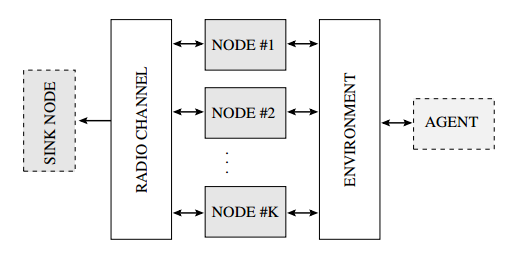
\includegraphics[scale=0.8]{netModel}
\caption{\label{netModel}Un modèle générique pour les RCSFs}
\end{figure}

\subsection{Le modèle du réseau}
\subsubsection{Les nœuds capteurs(nodes)}
chaque nœud capteur est un périphérique physique capturant un ensemble de grandeurs physiques.Les nœuds communiquent entre eux a l'aide d'un canal radio.a l'intérieur de chaque nœud, une pile de protocoles semblable a celle du modèle OSI contrôle la communication.A l'encontre des modèles classiques des réseaux sans fils,les nœuds capteurs incluent un second groupe de composants qui sont les unités de capture(qui capturent les grandeurs physiques) et qui sont connecter a l'environnement pour la détection de stimulus.

Les nœuds sont positionnés dans un environnement a deux ou a trois dimensions,un composant topologique additionnel(le composant de la mobilité) gère les coordonner du nœud dans l'environnement.Selon l'application,Le nombre de nœuds capteurs dans un RCSF  peut aller de quelques nœuds jusqu'à plusieurs milliers de nœuds.
\subsubsection{L'environnement}
Ce composant simule la génération et la propagation d' événements(les stimulus) qui sont détectés par les nœuds capteurs et qui déclenche une réaction de ces derniers(généralement une série de communication entre les nœuds du réseau).Les événements sont des grandeurs physiques comme du son,des ondes séismiques ou de la température.
\subsubsection{Le canal radio}
Le canal radio  simule la propagation des signaux radio entre les nœuds du réseau.Les modèles les plus détaillés incluent un composant de terrain ,qui simule un vrai terrain avec les obstacles qui peuvent y figurer et qui est connecté a l'environnement et au canal radio.Ce composant est pris en considération lors du calcule de la propagation des signaux dans le canal radio et influence aussi les grandeurs physiques mesurées.

\subsubsection{Les stations de base(sink nodes)}
Ce sont des nœuds spéciales qui ,s'ils sont présents ,reçoivent des données a partir des nœuds du réseaux et les traite(les agrège).Ils peuvent aussi envoyer des requêtes aux nœuds capteurs
afin de les interroger sur un événement particulier.L'utilisation des stations de base ou pas dépend de l'application qu'on veut mettre en place et des testes que l'on veut effectuer a l'aide du simulateur.

\subsubsection{Les agents}
Responsables de la génération des événements a destination des nœuds capteurs.Les agents peuvent causer une variation dans une grandeur physique,qui va se propager dans l'environnement et qui va stimuler les nœuds capteurs.Ce composant est utile lorsque son comportement peut être implémenté indépendamment de  l'environnement.Par exemple, un véhicule en mouvement,autrement,l'environnement lui même peu générer des événements. 

\subsection{Le modèle du nœud}

\begin{figure}[!h]

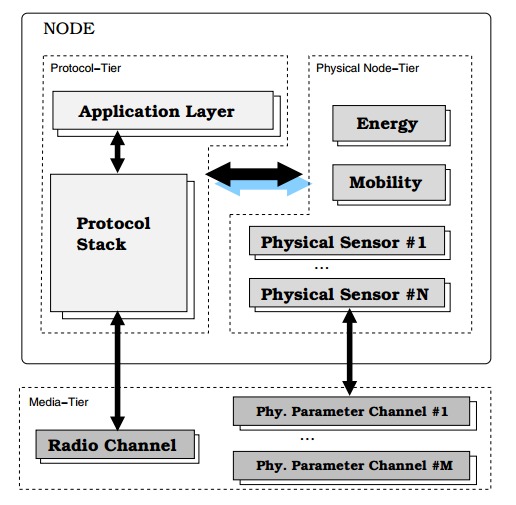
\includegraphics[scale=0.7]{nodeModel}
\caption{\label{nodeModel} L'architecture d'un nœud capteur}
\end{figure}

L'architecture du nœud peut être décomposée en trois tiers comme illustré dans la figure \ref{nodeModel}.
\begin{enumerate}
\item \textbf{Le tiers des protocoles:} 
Ce tiers comprend tout les protocoles de communications,typiquement,
trois couche coexistent dans ce niveau,la couche MAC,la couche de routage,et la couche application.Les opérations effectuées par ce tiers dépendent généralement de l'état du tiers physique décrit ci-dessous,par exemple, la couche réseau (la couche responsable du routage) peut prendre en considération les contraintes de la batterie pour décider de la route que va prendre le paquet.D'où,une méthode efficace d'échange d'informations entre les différents tiers doit être mise en place. 
\item\textbf{Le tiers physique}
Représente la plateforme matériel et ses effets sur les performances du nœud capteur.La composition de ce tiers peut changer suivant l'application implémentée par le nœud,les éléments les plus communs de ce tiers sont: un ensemble d'unités de capture(le capteurs physiques),le module de gestion énergétique et le module de gestion de la mobilité du nœud.Les capteurs physiques simulent le comportement du matériel de surveillance et de détection de stimulus.Le module énergétique simule la consommation énergétique du nœud,et le module de mobilité contrôle la position du nœud capteur dans l'environnement.
\item\textbf{Le tiers du média de transmission}
C'est le lien du nœud avec le monde extérieur.Un nœud est connecté avec l'environnement par le bais d'un canal radio(pour la communication avec les autres nœuds du réseau),et d'un ou plusieurs canaux physiques (pour la réception des événements ou stimulus a partir de l'environnement).
\end{enumerate}


\section{Les simulateurs des RCSFs}

L'accroissement de la recherche dans le domaine des RCSFs,spécialement dans ces dernières années, a conduit au développement d'une multitude de simulateurs pour les RCSFs.Les simulateurs peuvent êtres des framework(extensions) pour des outils de simulation existants (comme les framework Castalia et Mixim qui sont des extensions pour Omnet++), ou des simulateurs créés explicitement dans le but de simuler les RCSFs (comme TOSSIM).


\subsection{Type de simulateurs}
Il existe trois types de simulateurs selon le niveau de détail qu'ils emploient pour simuler les RCSFs.

le premier type sont les simulateurs a usage générale qui se concentrent sur des aspects de haut niveau des RCSFs comme le routage,la détection des stimulus,le traitement de l'information, et ignorent les aspects liés au système d'exploitation du nœud et a  son architecture matériel.Ce type de simulateur est pratique pour l'évaluation des protocoles et des algorithmes de haut niveau.Un exemple de ce type de simulateurs est Castalia.

Le second type sont les simulateurs niveau code qui permettent de développer des applications pour les RCSFs en utilisant le langage de programmation natif utilisé pour développé des application pour ce type de capteurs dans la réalité.Par exemple,le simulateur TOOSIM permet le développement d'applications pour les RCSFs en utilisant le langage de programmation NESC qui est le même utilisé dans la pratique pour développé des applications pour les capteurs de la marque MICA2.
Ce type de simulateur fait abstraction de l'architecture matériel du nœud et ne la prend pas en compte.Le code source de l'application et celui du système d'exploitation des nœuds capteurs simulés sont compilé suivant le code machine de la machine qui exécute le simulateur.Ce type de simulateur peut être utilisé pour la détection de bugs au niveau applicatif.

Le troisième type de simulateurs sont les simulateurs niveau firmware (ou niveau instruction machine).Ce type de simulateurs prend en compte l'architecture matériel du nœud capteur,et permet d'émuler un processeur comme celui trouvé dans de vrais nœuds capteurs et avec le même jeu d'instruction.De ce fait, les application développées dans ce type de simulateurs sont compilées suivant le code machine du nœud capteur simulé.
Utilisant ce type de simulateurs, la plupart des bugs peuvent être détectées, et les applications a contraintes temporelles peuvent être testées.

\subsection{Évaluation des simulateurs}
Pour pouvoir évaluer et comparer les différents outils de simulation existants, des critères d'évaluation doivent être établies.Les critères les plus pertinents sont:
\begin{itemize}
\item La disponibilité et la réutilisabilité;
\item La performance et la scalabilité;
\item Le support de langages de programmation riche en fonctionnalités pour définir les expérimentations et traiter les résultats;
\item Le support d'une interface graphique et d'un environnement de débogage.
\end{itemize}

Nous allons détailler chaque critère cité précédemment, en évaluant son impacte sur le choix d'un outil de simulation.

\subsubsection{Disponibilité et réutilisabilité}
Il y'a deux aspects clés a considérer ici:
\begin{itemize}
\item Est ce que l'outil de simulation inclue l'implémentation des modèles fréquemment utilisés dans la pratique (par exemple les modèles des protocoles MAC existants);
\item Avec quelle facilité pouvant nous modifier un modèle existant ou intégrer un nouveau modèle avec ceux déjà existants dans le simulateur.
\end{itemize}

La première question dépend de la durée de temps pendant laquelle le simulateur existe, et de la taille de la communauté qui l'utilise.Plus la communauté d'un simulateur est grande ,plus il y'aura des modèles disponible pour ce simulateur, et il est fort probable que s'il y'a de nouvelles propositions de modèles,celles-ci seront intégrées dans les prochaines versions du simulateur en question.

Dans le même contexte,il faudrait citer que tout les simulateurs incluent une implémentation plus ou moins complète de la pile de protocole TCP/IP, et doivent aussi inclure:
\begin{itemize}
\item Une implémentation des protocoles de routage communément utilisés dans les RCSFs;
\item Une implémentation des protocoles MAC communément utilisés  dans les RCSFs;
\item Une implémentation des modèles de propagation et de mobilité.
\end{itemize}

Par exemple,ces éléments sont généralement implémentés dans les simulateur des RCSFs:
\begin{itemize}
\item Le protocole de routage AODV;
\item Le protocole MAC IEEE 802.11;
\item Un modèle d'affaiblissement de propagation des signaux radios sur le canal de transmission.

\end{itemize}

La deuxième question est intimement liée a la conception du simulateur.Une structure étudiée, avec des interfaces bien définies, et une haute modularité, permet a l'utilisateur de facilement rajouter ou changer une fonctionnalité au simulateur.La disponibilité de modèles prêts a l'emploi, permet a l'utilisateur de rapidement mettre en place des scénarios de simulation, et de se concentrer sur des aspects plus spécifiques et plus importants dans la modélisation des RCSFs.
\subsubsection{Performance et scalabilité }
La performance et l'évolutivié sont deux problématiques majeurs dans le domaine de simulation des RCSFs.la première est généralement liée a l'efficacité du langage de programmation avec lequel le simulateur est développé.La deuxième est liée a la disponibilité de la mémoire vive, a la capacité de calcule du processeur et a la taille nécessaire pour stocker les fichiers log de la simulation.
\subsubsection{Support des langages de programmation riches en fonctionnalités}
La configuration typique d'une simulation d'un RCSF requiert de spéci fier au minimum les paramètres suivants:
combien de nœuds existent-ils dans la simulation?qu'elle est la position de chaque nœud?est-ce-que les nœuds sont mobiles?si oui,comment s'effectue ce mouvement?quel est le modèle énergétique utilisé ?combien de grandeurs physiques existent-elles dans la simulation?comment les événements sont-ils générés?quelle est la grandeur physique que doit détecter chaque nœud?qu'elles statistiques doit-on mesurer dans l'expérimentation?quels sont les paramètres du canal radio (canal de transmission)?.

Le nombre considérable de variables intervenant dans une simulation requiert l'utilisation d'un langage de programmation approprié avec des sémantiques de haut niveau  qui facilitent la définition des  paramètres de la simulation.
\subsubsection{Support d'une interface graphique et d'un environnement de débogage}
L'interface graphique est un outil intéressant dans les simulations pour les trois raisons suivantes:
\begin{itemize}
\item Elle constitue Une aide pour le débogage:  la façon la plus rapide et la plus pratique de détecter une anomalie dans le système simulé est de visualiser et de suivre le comportement de la simulation pas par pas.La caractéristique clé qu'une interface graphique devrait supporter est la capacité d'inspection des différents modules,des variables, et des files d'attentes des événements en temps réel(pendant l'exécution de la simulation).Ces caractéristiques rendent les interfaces graphiques des outils très puissants pour le débogage;
\item L'interface graphique peut servir comme outil de modélisation et de composition graphique:
cette caractéristique permet de faciliter et d'accélérer la construction de modules basiques, et la mise en place de petites expérimentations,cependant,pour les simulations volumineuses(avec un grand nombre de nœuds) l'approche graphique n'est pas très appropriée.
\item L'interface graphique peut inclure des outils pour la visualisation des résultats de la simulation( même en temps réel).
\end{itemize}

\subsection{Présentation de quelques outils de simulation existants}
Dans cette section on va présenter quelques simulateurs des RCSFs utilisés dans la pratique.Notre décision de choisir ces simulateurs est justifiée par les raisons suivantes:
\begin{itemize}

\item On a choisis les simulateurs gratuits et open source les plus utilisés dans le domaine de la recherche (surtout la recherche académique).
\item Dans le cas des simulateurs propriétaires(payants),on a choisis ceux dont les fournisseurs assurent le support activement.

\end{itemize}

En se basant sur ces critères on a choisis quatre simulateurs :ns-2,Castalia (qui se base sur omnet++),TOSSIM,COOJA/MSPSim.

NS-2 est le simulateur de réseaux le plus populaire,OMnet++ se distingue par une popularité croissante,une grande communauté et possède une structure modulaire ce qui a permit a la communauté de chercheurs de l'enrichir avec beaucoup de modèles et de fonctionnalités et lui donne le potentiel d'évoluer encore plus.TOOSIM est un simulateur de TinyOS,le système d'exploitation le plus utilisé dans les RCSFs.COOJA/MSPSim,sont des simulateurs du système d'exploitation Contiki avec sa popularité croissante. 

%INERNET OF THINGS%
  
 \subsubsection{NS-2}
NS-2 est le simulateur des réseaux le plus utilisé.Il a commencé comme un simulateur de réseaux de communication classiques,le support pour les réseaux ad hoc mobile(MANET) a été rajouté ultérieurement.NS-2 est un simulateur a événement discret ,orienté-objet, écrit en c++.Il dispose d'un interpréteur de langage OTCL utilisé comme front end.

Le noyau de simulation(le kernel),les modèles,les protocoles et les différents composants sont implémentés en c++,mais sont aussi accessible depuis OTCL.Les scripts OTCL sont utilisés pour la configuration du simulateur,la mise en place de la topologie du réseau, la spécification des scénarios de simulation,l'enregistrement des résultats de la simulation etc.Un script OTCL typique pour une simulation d'un réseau sans fils commence avec une commande de configuration qui définie les paramètres de la couche physique,de la couche MAC ,de  la couche de routage,du modèle de propagation radio etc.
L'étape suivante est la création des nœuds,les modèles de mouvement des nœuds et du trafic du réseau sont généralement définis dans des fichiers séparés et des outils sont disponibles pour la génération automatique de ces fichiers.

Un modèle très simple de consommation énergétique est utilisé.Chaque nœud démarre avec une quantité d'énergie initiale,les quantités d'énergies dépensées lors de la transmission et la réception de paquets sont aussi définies.Après l'envoi ou la réception d'un paquet,l'énergie du nœud est décrémentée par une certaine quantité.Quand l'énergie du nœud atteint zero, le nœud en question ne pourra ni envoyer ni recevoir de nouveaux paquets  

L'outil nam permet la visualisation graphique de la progression de la simulation.Durant la simulation ,NS-2 génère un fichier  contenant la trace de la simulation destiné a nam,un script OTCL est utilisé pour définir quelles informations devraient être enregistrées dans ce fichier.Nam utilise les données stockées dans ce fichier pour donner une visualisation de la topologie du réseau,et pour animer la circulation des paquets.

L'utilisation de NS-2 comme outil de simulation pour les RCSFs possède ses inconvénients:d'abord, il n'existe pas  de modèles pour les capteurs physiques(les unités de capture),de plus, les formats de paquets et les protocoles MAC définies dans NS-2 sont différents de ceux qu'on trouve dans les RCSFs et le modèle de consommation énergétique est très simple.

Cependant,NS-2 est extensible et plusieurs extensions tiers on été développées pour combler les manques cités précédemment.MANNASIM ajoute par exemple: un modèle de capteurs physiques,beaucoup de modèles d'applications,une implémentation du protocole de routage LEACH,un modèle des capteurs de la marque MICA2 et une interface graphique pour créer automatiquement des scripts OTCL.

\subsubsection{Omnet++ et Castalia}
Un autre simulateur a événements discrets est Omnet++.Ce n'est pas un simulateur spécifique aux réseaux de capteurs et ce n'est pas non plus un simulateur spécifique aux réseaux de communications,mais une plateforme pour le développement de simulateurs dans laquelle plusieurs groupes peuvent construire leur propres simulateurs.Comme l'utilisation la plus répandu d'Omnet++ est la construction de simulateurs pour les réseaux de communication,il est communément décrit comme un simulateur de réseaux.

Un simulateur basé sur Omnet++ est construit a partir d'éléments appelés modules.Les modules simples ou \emph{simple modules}(leur appellation dans le vocabulaire d'Omnet++) sont les briques de base de la simulation et leur comportement est définie avec du C++.Les modules composés ou \emph{Compound modules} sont obtenues par l'imbrication d'autres modules (simples ou composés) liés entre eux par des connexions.Le Module composé de plus haut niveau est le réseau (\emph{network module}).

Les différents modules communiquent entre eux a l'aide de messages, qui sont soit envoyer a travers la chaine de connexions entre les modules,soit  directement a partir d'un module vers un autre.
La définition des modules simples,des modules composés et de la topologie du réseau est réalisée en utilisant un langage déclaratif appelé NED.Les paramètres de la simulation sont définit dans un fichier de configuration(généralement nommé omnetpp.ini ).

OMNET++ inclue un environnement de développement intégré (IDE) basé sur l'IDE eclipe, qui simplifie  la programmation des modules en offrant un support pour le langage C++,il offre aussi un support pour la rédaction des fichiers NED(fichiers avec extension ".ned") et des fichiers de configuration (fichiers avec extension ".ini") en intégrant des outils pratiques comme la colorisation des mots clés,l'auto-complétion,le débogage des programmes C++ etc.

Tkenv est le nom de l'interface graphique utilisée pour l'exécution de la simulation.C'est un outil très puissant qui permet de visualiser  l'exécution de la simulation en représentant la circulation des messages entre les nœuds du réseau avec des animations.Elle permet aussi la visualisation du changement d'état de chaque objet dans la simulation , la visualisation des résultats de la simulation et l'analyse de ces derniers.

Un exemple de simulateurs de RCSFs construit avec Omnet++ est Castalia .C'est un simulateur de haut niveau prévu pour faire le test et la validation des algorithmes de haut niveau(algorithmes de routage,algorithmes de la couche MAC) avant de passer a leurs implémentation sur une plateforme spécifique.
\begin{figure}[!h]
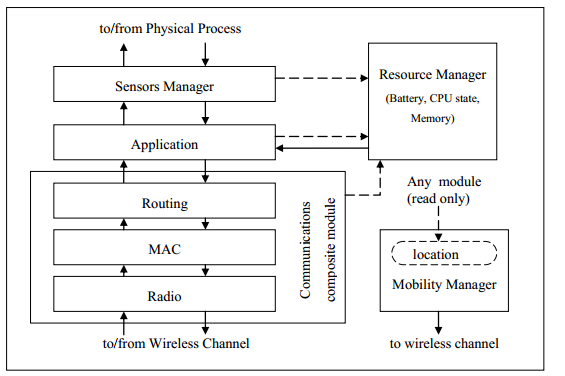
\includegraphics[scale=0.8]{castaliaModel}
\caption{\label{castaliaModel}Le Modèle d'un nœud capteur dans Castalia}
\end{figure}
Dans Castalia, les nœuds capteurs sont implémentés comme des modules composés \emph{Compound modules}, constitués d'un ensemble de sous modules qui représentent:
\begin{itemize}
\item La pile des protocoles de communication (MAC ,routage);%(communication module);
\item L'application;
\item Les capteurs physiques(\emph{sensors manager});
\item L'antenne radio (émetteur/récepteur des signaux radios);
\item Le gestionnaire de ressources qui incluent la batterie ,le processeur ,et la mémoire,et qui communique avec tout les autres modules;
\item Le gestionnaire de mobilité qui s'occupent de gérer la mobilité du nœud et sa position dans l'environnement.
\end{itemize}

Le module radio \iffalse (communément appelé module physique ou \emph{PHY module}) \fi simule le comportement d'une antenne radio basse puissance qui peut prendre différents états (chaqu'un d'eux travail avec une différente consommation énergétique) et différents niveaux de puissance de transmission.Le module radio effectue aussi La détection de la porteuse et la modulation,les modulations de type PSK et FSK sont supportés et l'utilisateur peut très bien définir ses propres modèle de modulation.

Il y'a deux modules MAC disponible dans CASTALIA.
,le premier implémente les protocoles TMAC et SMAC alors que le deuxième peut réalisé une approximation de plusieurs protocoles MAC mais ne supporte que les communications en mode broadcast.Les modules radio et MAC peuvent être contrôlés a partir de l'application.

Les grandeurs physiques a détecter (les stimulus) sont modélisées par des processus physiques qui peuvent se déplacer et changer de valeur.Les effets de  bruit et de  diffusion sont pris en considération lors de la détection de ces grandeurs physiques.

Le modèle énergétique utilisé est très simple,il est comparable a celui utilisé par NS-2.

\subsubsection{TOSSIM}
TOSSIM est un simulateur niveau code,a événement discret, pour la simulation des nœuds capteurs qui utilisent TinyOS comme système d'exploitation(la plupart des nœuds capteurs existants).Au lieu de compiler une application pour TinyOS sur un vrai nœud capteur,l'utilisateur peut la compiler dans TOSSIM qui s'exécute sur un PC,et ceci permet a l'utilisateur de faire le test,le débogage et l'analyse des algorithmes dans un environnement contrôlable et reproduisible.

Le but principale de TOSSIM est de fournir une simulation aussi fidèle que possible des applications de TinyOS.Pour cette raison, il se concentre beaucoup plus sur la simulation de TinyOS et sur son exécution plutôt qu'a la simulation du monde réel.Bien que TOSSIM peut être utilisé pour comprendre les causes d'un comportement observé dans le monde réel,il ne peut pas capturer toutes les causes,et il ne doit par être utilisé pour faire des assertions absolues.

TOSSIM permet la simulation des applications de TinyOS en remplaçant quelques composants de bas niveau avec des implémentations de la simulation.C'est un simulateur a événements discrets ou les événements de la simulation représentent les interruptions matériels,les événements système et les taches a exécuter.

TOSSIM possède trois lacunes.D'abord,tout les nœuds simulés doivent exécuter la même application.De plus,TOSSIM ne prend pas en compte la consommation énergétique (bien qu'il existe l'extension "PowerTOSSIM" qui permet de régler ça).

\subsubsection{COOJA/MSPSim}
COOJA/MSPSim sont des simulateurs inclus dans la distribution du système d'exploitation pour les capteurs sans fils Contiki.MSPSim peut être intégré dans COOJA formant ainsi COOJA/MSPSim.

MSPSim est un simulateur niveau firmware basé sur le jeux d'instruction du microcontrôleur \emph{Texas Instruments MSP430}.Il combine l'interprétation des instructions CPU avec la simulation a événements discrets des autre composants.

COOJA est un simulateur niveau code pour les RCSFs avec des nœuds utilisant Contiki comme système d'exploitation.des nœuds avec différentes  plateformes matériels et exécutant différents applications peuvent coexister dans le même simulation.

La combinaison COOJA/MSPSim peut simuler des nœuds capteurs sur les trois niveaux de détails cités précédemment(haut niveau,niveau code,niveau firmware).De plus,des nœuds simulés sur différents niveaux de détails peuvent coexister et interagir dans la même simulation,
cette fonctionnalité est appelée \emph{cross level simulation} et est parmi les points forts de COOJA/MSPSim.

\section{Présentation d'Omnet++}
Comme notre travail est basé sur Omnet++ nous allons donner dans cette section une description de cet outil de simulation.

OMNET++ est un \emph{framework} orienté objet,modulaire, pour la simulation des réseaux.Il est basé sur la simulation a événement discret.

Omnet++ peut être utilisé (et il est utilisé ) dans divers domaines:
\begin{itemize}
\item La modélisation des réseaux filaires et des réseaux sans fils; 
\item La modélisation des protocoles;
\item La modélisation des architectures multiprocesseur et d'autres systèmes distribués;
\item La validation des architectures matériels;
\item D'une façon générale la modélisation et la simulation de n'importe quel système pouvant être simulé en utilisant l'approche de simulation a événements discrets, et qui peut être représenté par un ensemble d'entités communicants par l'échange de messages.
\end{itemize}

OMNET++, en lui même,n'est pas un simulateur d'un système en particulier,mais plutôt,il fournit une infrastructure et des outils pour le développement de simulateurs.

L'un des ingrédients fondamentaux de cette infrastructure est son architecture a base de composants,les modèles sont assemblés a partir de composants réutilisables appelés modules,les différents modules peuvent êtres interconnectés via leurs portes (\emph{gates}), et peuvent êtres imbriqués pour formé des modules composés.La profondeur de l'imbrication des modules n'est pas limité.

les modules communiquent par l'échange de messages et les messages peuvent transporter n'importe quelle structure de donnée.Les modules peuvent envoyé un message soit a travers un chemin prédéfini -formé d'une série de connexions entre les nœuds- ,ou directement a son destinataire (le dernier cas est particulièrement utile pour la simulation des communications sans fils).

Les modules peuvent contenir des paramètres qui sont utilisés pour personnaliser leur comportement et paramétrer la topologie du modèle.les modules au plus bas niveau de la hiérarchie(les modules atomiques) sont appelés modules simple(\emph{simple modules} dans le vocabulaire d'Omnet++) et il encapsulent le comportement du modèle. Les modules simples sont programmés en C++ et font usage de la librairie de simulation d'Omnet++.

Les simulations construites avec Omnet++ peuvent être exécutées avec divers interfaces utilisateur.Les interfaces graphiques contenant des animations sont très utiles pour le débogage de la simulation et l'inspection des différents modules.De l'autre coté ,les interfaces en ligne de commande sont utiles pour l'exécution par lots (batch processing).

OMNET++ supporte aussi les simulations parallèles distribuées,OMNET++ peut utilisé différents mécanismes pour la communication entre les différentes partitions d'une simulation parallèle distribué,par exemple MPI .Les modèles n'ont pas besoin d'une manœuvre (instrumentation) particulière  pour qu'ils puissent être exécuté en parallèle,c'est juste une question de configuration.
 
Le simulateur ainsi que les différents outils et interfaces sont très portables et sont testés dans la plupart des systèmes  d'exploitation (Linux,Mac OS/X,Windows) et ils peuvent être recompilé (après modification) dans la plupart des système basés sur Unix.

\subsection{Concepts de modélisation }
\subsubsection{Généralités}
Un modèle dans Omnet++ consiste en un ensemble de modules qui communiquent entre eux avec des messages.Les modules actifs sont les modules simples et leur comportement est définie avec du C++ en utilisant la librairie de simulation.Les modules simples peuvent être groupés pour construire des modules composés.Le réseau finale obtenue est  un module composé.

La figure \ref{simpleCompound} représente des modules simple(arrière plan gris) et des modules composés.Les flèches  représentent les connexions entre les différents modules,a travers les portes de ces derniers.

\begin{figure}[!h]
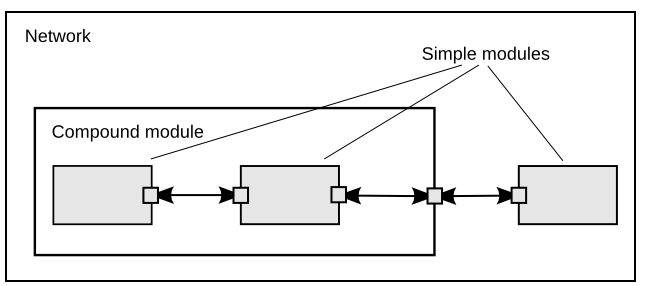
\includegraphics[scale=0.7]{simpleCompound}
\caption{\label{simpleCompound}Les modules simples et composés}
\end{figure}

					
Les modules communiquent entre eux  avec des messages qui peuvent contenir n'importe quelle donnée, en plus des attributs habituels tel que l'estampille du message.Les modules envoient les données généralement a travers leurs  portes,mais il est aussi possible de les envoyer directement vers le module de destination(sans passer par les portes).Les portes sont les interfaces d'entrée et de sortie des modules,les messages sont -généralement- envoyés a travers les portes de sortie et arrive sur les portes d'entrées.

Une porte d'entrée d'un module et une porte de sortie d'un autre module peuvent êtres liées par une connexion,les connexion peuvent être créées entre modules appartenant au même niveau hiérarchique :Dans un modules composé,les portes de deux sous-modules,ou une porte d'un sous-module et la porte du module composé parent peuvent être interconnectées.Les connexions impliquant des modules appartenant a différents niveaux hiérarchiques ne sont pas permises car ça constituerait un obstacle pour la réutilisation du modèle.

A cause de la structure hiérarchique du modèle les messages passent généralement par une chaine de connexions partant de et arrivant dans des modules simples,Les modules composés agissent comme des conteneurs dans le modèle, faisant office de relai de messages entre leur sous-modules et le monde extérieur.Des paramètres comme le délai de propagation,le débit de transfert de données et le taux d'erreurs peuvent êtres assignées aux connexions.

L'utilisateur peut définir des types de connexions avec leur propriétés spécifiques ,ces types de connexions sont appelées -dans le vocabulaire d'Omnet++- les \emph{Channels} (pour canaux de communication)  et peuvent être réutilisé dans plusieurs endroits de la simulation.

Les modules peuvent avoir des paramètres,les paramètres sont principalement utilisés pour passer des données de configuration aux modules et pour aider a définir la topologie du modèle.Les paramètres peuvent êtres  de différents types: des chaines de caractères,des types numériques ou des booléens,les paramètres peuvent aussi agir comme des sources de nombres aléatoires dont la distribution est définie dans les fichiers de configuration du modèle,leurs valeurs peuvent aussi êtres assignées d'une façon interactive par l'utilisateur lors de l'exécution de la simulation.Les paramètres peuvent  contenir des expressions référençant d'autres paramètres et les modules composés peuvent passer des paramètres ou des expressions a leur sous modules.

Omnet++ fournit des moyens  pour permettre a l'utilisateur de décrire  la structure du système d'une façon efficace,les principaux sont les suivants:

\begin{enumerate}
\item Un langage de description de la topologie;
\item L'imbrication hiérarchique des modules;
\item La définition de différents types de modules et de connexions;
\item Une flexibilité dans la définition des paramètres des modules;
\item Une communication entre les modules a l'aide de messages.
\end{enumerate}

\subsubsection{Imbrication des modules}
Un simulateur construit avec Omnet++ consiste en un ensemble de modules hiérarchiquement imbriqués qui communiquent en s'envoyant des messages.Tout commence avec les modules simples qui sont les briques de bases.Ensuite, après une série  d'imbrication(le nombre d'imbrication est illimité) et d'interconnexion des modules, on obtient le réseau désiré.
La définition des modules,des interconnexions et de la topologie du réseau est réalisée avec le langage NED.

\subsubsection{Types de modules/Types de connexions }
Ici l'analogie est faite avec la programmation orienté objet,dans laquelle on définie des types(des classes) ensuite on les instancie pour construire le système désiré.

tout les modules ,simples ou composés, sont des instances de types de modules.Dans la description du modèle,l'utilisateur définie des types de modules.Les instances de ces types peuvent servir comme composants afin de construire des types de modules encore plus complexes.

Les types de modules peuvent être stockés dans des fichiers séparés de l'emplacement de leur utilisation.Cela veut dire que l'utilisateur peut regrouper plusieurs types de modules existants, et ainsi, construire des bibliothèques de composants.

Le même raisonnement s'applique pour les connexions entre les nœuds.Bien qu'il existe des types de connexions prédéfinies dans Omnet++ que L'utilisateur peut utiliser directement,l'utilisateur peut très bien définir des types de connexions  personnalisés et leur assigné des paramètres comme le délai de propagation,le débit de transfert des données etc.Ces types de connexions peuvent être instanciés par la suite dans différents endroits de la simulation. 
\subsubsection{Les messages}
Les modules communiquent en s'échangeant des messages.Dans une simulation,les messages peuvent être des trames ou des paquets dans le cas d'un réseau d'ordinateurs,des travaux(jobs) ou des clients dans une file d'attente, ou autre type d'entités mobiles.

Le temps local de simulation d'un module avance quand le module reçoit un message.Le message peut arriver d'un autre module ou du module lui même.Dans le deuxième cas,le module s'auto envoi un message,et ceci permet l'implémentation des timer (quand le timer expire le module effectue une action).
\subsubsection{Modélisation de la transmission du paquet}
Afin de modéliser les réseaux de communication,
les connexions sont utilisées pour modéliser les liens physiques.Les connexions supportent les paramètres suivants:
\begin{itemize}
\item Le débit de transfert des données;
\item Le délai de propagation;
\item Le taux d'erreurs de transmission que se soit au niveau des bits ou au niveau des paquets.
\end{itemize}

Quand le débit de transfert des données est spécifié,le paquet est par default délivré au module cible au temps de la simulation qui correspond a la fin de la réception de ce dernier.Vu que ce comportement n'est pas convenable pour la modélisation de quelques protocoles(half duplexe ethernet),OMNET++ offre la possibilité au module de destination de spécifier que le paquet doit lui être délivré quand la réception commence.
\subsubsection{Les paramètres}
Les modules peuvent avoir des paramètres,ces paramètres peuvent être assignés  soit dans les fichiers ".ned",soit dans le fichier de configuration  "omnetpp.ini".
Les paramètres peuvent être utilisés pour personnaliser le comportement des modules  et pour paramétrer la topologie du modèle.
Les paramètres peuvent avoir comme valeurs des chaines de caractères,des valeurs numériques,des valeurs booléennes,et même des fichier XML.Les valeurs numériques  peuvent êtres: des expressions utilisant d'autres paramètres et/ou appelant des fonctions prédéfinies,des variables aléatoires de différentes distributions  ou des constantes introduites interactivement par l'utilisateur.

Les paramètres a valeurs  numériques peuvent êtres utilisés pour construire des topologies d'une manière flexible.Au sein d'un module composé, les paramètres peuvent être utilisés pour paramétrer les sous-modules .Ainsi, ils peuvent être utilisés pour définir le nombre de sous modules,le nombre de portes de ces derniers, et la façon avec laquelle les connexions entre les sous modules sont effectuées.

\subsubsection{Méthode de description de la topologie}
La topologie du réseau est définie dans les fichiers ".ned" ceci inclue:
\begin{itemize}
\item La définition des différents types de modules intervenants dans la simulation et la spécification de leurs paramètres;
\item La définition des différents types de connexions intervenants dans la simulation et la spécification de leurs paramètres;
\item L'interconnexion des différents modules via leurs portes en spécifiant les types de connexions utilisés;
\item L'imbrication des modules pour construire de nouveaux types de modules(selon l'application et les tests que l'on veut réaliser);
\item La construction du réseau globale en instanciant les modules définies précédemment et en effectuant les interconnexions nécessaires.  
\end{itemize}

\subsection{Programmation des algorithmes}

Les modules simples sont la partie actif du modèle, leur comportement est définie en utilisant le langage de programmation C++.Si l'utilisateur veut définir un algorithme de routage,un algorithme de la couche MAC ou n'importe quel autre fonctionnalité, il doit créer un module simple pour ça, et implémenter l'algorithme voulue comme des fonctions en C++.
Toute la puissance du langage C++ peut être utilisée.Le programmeur de la simulation peut choisir librement entre un style de programmation événementiel ou un style de programmation procédurale classique. Et peut très bien utiliser tout les concepts de la programmation orienté objet (l'héritage,le polymorphisme,les design patterns etc).

Les objets présents dans la simulation(messages,modules,files d'attente etc) sont représentés par des classes implémentées en C++.Ces classes ont été conçues de façon a pouvoir travailler ensemble efficacement,créant ainsi  un framework puissant pour la programmation de simulations.Les classes suivantes font partie de la bibliothèque de simulation d'Omnet++:

\begin{itemize}

\item Module,gate,parameter,channel;
\item Message,packet;
\item Les classes contenaires (les files,les tableaux);
\item Les classes pour faire des statistiques(histogrammes,calcule des quantiles);
\item Les classes pour le calcule de la précision des résultats de la simulation.
\end{itemize} 

Les classes sont spécialement développées de façon a permettre l'inspection des objets(instances de ces classes) durant l'exécution de la simulation, et d'afficher des informations les concernant,comme le nom de chaque objet,le contenue de l'objet ,le nom de la classe a partir de laquelle l'objet a été instancié etc.Cette possibilité permet la création d'une simulation ou tout les composants internes et leurs propriétés sont visibles dans l'interface graphique.

\subsection{Les interfaces utilisateur}
L'objectif principale des interfaces utilisateur est de rendre l'intérieur du modèle(les composants du modèle) visibles a l'utilisateur, et de lui offrir la possibilité de changer les variables et les objets du modèle pour lui permettre de contrôler l'exécution de la simulation.L'interface graphique est un outil très important dans la phase du développement et du debogage de la simulation et sert a prouver que le modèle est fonctionnel.

La même simulation peut être exécutée avec différentes interfaces utilisateur et ceci  sans faire de modifications dans les fichiers du modèle,c'est juste une histoire de configuration.Ceci  permet  a l'utilisateur de faire le test et le débogage de la simulation avec  une interface graphique puissante, et finalement,d'exécuter la simulation avec une interface  utilisateur simple et rapide qui supporte l'exécution  par lots (batch excution).

\subsection{OMNET++ dans la pratique}

Omnet++ est composé des parties suivantes:

\begin{itemize}
\item \textbf{ Le noyau de la simulation:} Il contient le code qui gère la simulation et la librairie de classes de la simulation.Il est écrit en C++.
\item \textbf{ Les interfaces utilisateur}:Les interfaces utilisateur dans OMNET++ sont utilisées pendant l'exécution de la simulation pour faciliter le débogage  ,la démonstration, et les exécutions par lots (batch execution).Elle sont écrites en C++ et compilées sous forme de bibliothèques dynamiques.	
\end{itemize}

Un modèle dans OMNET++ est constitué des parties suivantes:
\begin{itemize}
	\item \textbf{La description de la topologie}:Elle se fait en utilisant le langage NED(les fichiers avec extension ".ned") ,qui est utilisé pour décrire la structure des modules en définissant leurs paramètres,leurs portes,les interconnexions etc.Les fichiers NED peuvent être rédigés en utilisant n'importe quel éditeur de texte.L'IDE d'Omnet++ fourni un excellent support pour l'édition de ces fichiers, soit d'une manière graphique en glissant/déposant des composants tout prêts,soit d'une manière textuel;
	\item\textbf{ La définition des types de messages utilisés dans la simulation:}Ceci se fait dans des fichiers avec extension ".msg";OMNET++ permet de définir plusieurs types de messages  et de leurs ajouter des champs de données qui représentent alors le contenu de ces messages.OMNET++ va par la suite généré automatiquement des classes en C++ a partir de ces définitions pour que ces types de messages puissent être instanciés et utilisés par a suite dans la simulation.
	\item \textbf{Le code source des modules simples:}Les modules simples sont la partie actif du modèle,leurs implémentation est faite en C++(dans les fichiers ".cc/.h").Cette implémentation décrit la tache réalisé par ces modules simples.
\end{itemize}	

Les programmes de simulation sont construits a partir des composants cités précédemment.D'abord les fichiers ".msg" contenant la définition des messages sont traduit
en C++ en utilisant le programme $opp_msgc$ fournit avec Omnet++.Ensuite,les fichiers 
sources en C++ sont compilés et une édition de liens est effectuée avec la noyau de la simulation et avec une interface utilisateur pour former soit un exécutable de la simulation(un simulateur) et dans ce cas il pourra être exécuté sur une machine même si celle ci ne dispose pas d'Omnet++,soit une bibliothèque dynamique et dans ce cas les bibliothèques d'Omnet++ doivent être présentes dans la machine ou cette bibliothèque dynamique est utilisée.Les fichiers NED et le fichier de configuration "omnetpp.ini" sont chargé dynamiquement sous leur forme textuel quand la simulation est exécutée.

L'exécutable de la simulation peut inclure plusieurs modèles indépendants qui utilisent le même ensemble de modules.L'utilisateur peut spécifier dans le fichier de configuration quel modèle il désire exécuter.Ceci permet de créer un large exécutable qui contient plusieurs modèles de simulation,et de le distribuer comme outil de simulation autonome.La flexibilité dans la description de la topologie contribue a la réalisation de cette fin. 

Quand l'exécutable de la simulation est lancé ,il lit d'abord tout les fichier NED contenant la topologie du modèle,ensuite il lit le fichier de configuration (généralement appelé omnetpp.ini),ce fichier contient les paramètres qui contrôlent comment la simulation sera exécuter,et fournie les valeurs au paramètres des différents modules.Le fichier de configuration peut aussi indiquer que la simulation doit s'exécuter plusieurs fois,dans le cas le plus simple, les exécutions se feront l'une après l'autre, avec les mêmes paramètres  ou avec des paramètres différents a chaque exécution.

Les résultats de la simulation peuvent être sauvegardés dans des fichiers.Il existe deux formats de fichier prédéfinies dans OMNET++ pour la sauvegarde des résultats de la simulation: les \emph{vector files} qui servent a l'enregistrement des résultats au fur et a mesure de l'exécution de la simulation (enregistrement a intervalle de temps régulier),et les \emph{scalar files} qui servent a enregistrer des statistiques a la fin de l'exécution de la simulation.L'utilisateur peut définir ses propres formats de fichiers pour la sauvegarde des résultats.L'IDE fournit avec Omnet++ offre un environnement riche pour l'analyse de ces fichiers de résultat.

\section{Présentation de Castalia}
Castalia est un simulateur pour les RCSFs,les réseaux BAN (Body Area Nerworks),et plus généralement les réseaux contenants des dispositifs travaillant a une faible puissance.

Castalia est basé sur Omnet++ et peut être utilisé pour tester les algorithmes/protocoles  distribués, en offrant des modèles réalistes du canal de communication sans fils et de la transmission radio,avec un comportement réaliste des nœuds capteurs.
De plus,vu qu'il est hautement paramétrable ,Castalia peut être utilisé pour tester l'influence de différents paramètres et caractéristiques sur le fonctionnement d'une application spécifique. 

Les principales caractéristiques de Castalia sont:

\begin{itemize}
\item Un modèle réaliste du canal de communication sans fils, basé sur des mesures empiriques
 	\begin{itemize}
 	\item Le modèle prend en compte la perte des 		   		  données du a leur transition sur le canal de			  communication
	\item Le modèle prend en compte la variation 				  temporelle de la perte des données
	\item Le modèle supporte la mobilité des nœuds
	\item Le modèle prend en compte l'interférence lors 		  du calcule de la puissance du signale reçu   
 	\end{itemize}
\item Un modèle détaillé de la transmission  radio basé sur des radios réels pour les communications a basse puissance
	\begin{itemize}
		
	\item La probabilité de la réception est basée sur le SINR,la taille du paquet et le type de modulation(les modulations PSK et FSK sont supportées et l'utilisateur peut définir des schémas de modulation personnalisées)
	\item L'utilisateur peut définir différents niveaux de puissances de transmission,ces puissances peuvent varier d'un nœud a l'autre
	\item La possibilité de définir plusieurs états dans lesquelles un nœud capteur peut se trouver,avec différentes consommations énergétiques et des délai de commutation en eux
	\item Une modélisation réaliste de la détection de la porteuse  
	\end{itemize}
\item La prise en compte des dérives des horloges des nœuds
\item Inclue une implémentation des protocoles MAC et des protocoles de routage communément utilisés dans le domaine des RCSFs
\item Castalia a été conçue de façon a ce qu'il soit extensible
\end{itemize}

Concernant la dernière caractéristique,la conception de Castalia permet aux utilisateurs de facilement implémenter leur propres algorithmes et protocoles tout en faisant usage des caractéristiques qu'offre le simulateur.La modularité,la rapidité,et l'efficacité de Castalia est principalement du a Omnet++.

Castalia n'est pas un simulateur spécifique a une plateforme matériel particulière des nœuds capteurs, mais plutôt un outil pour le test et la validation des algorithmes de haut niveau avant leurs implémentation sur une plateforme matériel particulière.
\subsection{Structure de Castalia}
La figure \ref{basicStructCastalia} montre l'architecture basique d'un RCSFs dans Castalia.
\begin{figure}[!h]
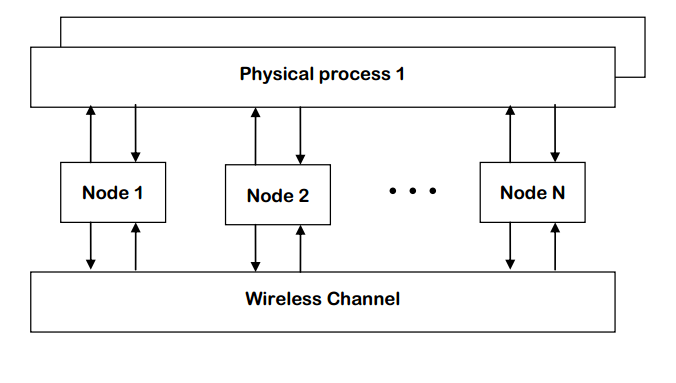
\includegraphics[scale=0.7]{basicStructCastalia}
\caption{\label{basicStructCastalia} Les modules et leurs connexions dans Castalia}
\end{figure}

Les modules ne sont pas connectés directement mais a travers le module qui représente le canal de communication sans fils.Les flèches représentent le transfert de messages entre les nœuds du réseau.Quand un nœud transmet un paquet,ce dernier passe par le canal de communication sans fils qui décide alors quels nœuds devraient le recevoir.Les nœuds sont aussi liés par les processus physiques(grandeurs physiques) qu'ils sont entrain de surveiller.Chaque processus physique est modélisé par un module qui détient la quantité de la grandeur physique représentée par ce processus physique.Les nœuds échantillonnent les processus physiques( en envoyant un message au module correspondant) pour obtenir leurs lectures.Il peuvent y avoir plusieurs processus physiques dans une simulation.

Le nœud capteur est un module composé,la figure \ref{castaliaModel} dans la page \pageref{castaliaModel} montre la structure interne d'un nœud.Les flèches en gras représentent des transferts de messages tandis que les flèches en pointillé représentent des appelles de fonctions.Par exemple, la plupart des modules appellent une fonction du gestionnaire de ressources pour signaler que l'énergie a été consommée.

tout les modules existants (application,routage,Mac,etc) sont hautement configurables, et peuvent être changés par l'utilisateur en créant de nouveaux modules afin de définir une nouvelle application,un nouveau protocole de routage,un nouveau modèle de mobilité etc.


%\chapter*{Conclusion générale}

%\chapter*{Annexe}

\bibliographystyle{authordate1} 
\bibliography{Bibliographie/BibliographieBDD}


					
					
%-----------------fin de la numerotation avec les chiffres arabs---------------------

\end {document}